\documentclass[12pt]{article}
\usepackage{amssymb}
\usepackage{amsthm}
\usepackage{dsfont}
\usepackage{amsmath}
\usepackage[latin1]{inputenc}
\usepackage[english]{babel}
\usepackage{graphicx}
\usepackage{bbm}
\usepackage{tikz}
\usepackage{color}  
%\usepackage{nath}
%\delimgrowth=1

\usepackage[margin=1in,footskip=0.25in]{geometry}
\linespread{1.3}

\usepackage{verbatim}
\usepackage{enumitem}

\newtheorem{theorem}{Theorem}%[section]
\newtheorem{lemma}[theorem]{Lemma}
\newtheorem{proposition}[theorem]{Proposition}
\newtheorem{corollary}[theorem]{Corollary}
\newtheorem{question}{Open question}
\newtheorem{defi}[theorem]{Definition}
\theoremstyle{plain}
\newtheorem{assumption}{Assumption}

\theoremstyle{remark}
\newtheorem{remark}{Remark}
\newtheorem{example}{\it Example\/}

\theoremstyle{definition}
\newtheorem{exercise}{Exercise}
\newtheorem{problem}{Problem}

\def\RRn{\mathbb{R}^n}
\def\RR{\mathbb{R}}
\def\RRN{\mathbb{R}^N}
\def\ZZ{\mathbb{Z}}
\def\ZZN{\mathbb{Z}^N}
\def\RRnm{\mathbb{R}^{n \times m}}
\def\RRmn{\mathbb{R}^{m \times n}}

\def\dd{\, \mathrm{d}}

\def\grad{\nabla}
\def\weakConv{\rightharpoonup}
\def\LL{\mathrm{L}}
\def\WW{\mathrm{W}}
\def\naturals{\mathbb{N}}

\def\intRRn{\int_{\RRn}}

\def\calM{\mathcal{M}}
\def\calE{\mathcal{E}_p}
\def\calC{\mathcal{C}}

\def\dist{\text{dist}}
\def\supp{\text{supp}}
\def\indyk{\mathds{1}}

\def\intOmega{\int_{\Omega}}
\def\intRRnm{\int_{\RRnm}}

\def\PP{\mathrm{P}}

\def\Ccinfty{C_c^{\infty}}

\DeclareMathOperator{\im}{Im}
\DeclareMathOperator{\id}{Id}
\renewcommand{\phi}{\varphi}
\renewcommand{\epsilon}{\varepsilon}
\renewcommand{\geq}{\geqslant}
\renewcommand{\leq}{\leqslant}
\renewcommand{\div}{\text{div}}

\newcommand{\measurerestr}{%
  \,\raisebox{-.127ex}{\reflectbox{\rotatebox[origin=br]{-90}{$\lnot$}}}\,%
}

\def\Xint#1{\mathchoice
{\XXint\displaystyle\textstyle{#1}}%
{\XXint\textstyle\scriptstyle{#1}}%
{\XXint\scriptstyle\scriptscriptstyle{#1}}%
{\XXint\scriptscriptstyle\scriptscriptstyle{#1}}%
\!\int}
\def\XXint#1#2#3{{\setbox0=\hbox{$#1{#2#3}{\int}$ }
\vcenter{\hbox{$#2#3$ }}\kern-.6\wd0}}
\def\ddashint{\Xint=}
\def\dashint{\Xint-}

\renewcommand{\phi}{\varphi}
\renewcommand{\epsilon}{\varepsilon}
\renewcommand{\geq}{\geqslant}
\renewcommand{\leq}{\leqslant}

\def\RRn{\mathbb{R}^n}
\def\RR{\mathbb{R}}
\def\RRN{\mathbb{R}^N}
\def\ZZ{\mathbb{Z}}
\def\ZZN{\mathbb{Z}^N}
\def\multiindices{\mathbb{Z}^N_+}
\def\RRnm{\mathbb{R}^{n \times m}}
\def\RRmn{\mathbb{R}^{m \times n}}
\def\naturals{\mathbb{N}}

\def\Ccinfty{C_c^{\infty}}

\def\dd{\, \mathrm{d}}
\def\grad{\nabla}
\def\weakConv{\rightharpoonup}

\def\intRRn{\int_{\RRn}}
\def\intOmega{\int_{\Omega}}
\def\intRRnm{\int_{\RRnm}}
\def\intRRN{\int_{\RRN}}

\def\RRNn{\RR^{N \times n}}

\def\CC{\mathrm{C}}

\def\RRn{\RR^n}
\def\RRm{\RR^m}

\usetikzlibrary{shapes, arrows, calc, arrows.meta, fit, positioning}  
\tikzset{  
    -Latex,auto,node distance =1.5 cm and 1.3 cm, thick,
    state/.style ={ellipse, draw, minimum width = 0.9 cm}, 
    point/.style = {circle, draw, inner sep=0.18cm, fill, node contents={}},  
    bidirected/.style={Latex-Latex}, 
    el/.style = {inner sep=2.5pt, align=right, sloped}  
}  

\def\hint{\noindent \textbf{Hint: }}
\begin{document}

\begin{center}
\begin{Large}
\textbf{LN fee bounds: Interest Return and Transaction Fee}

\end{Large}
\text{sketch}
\end{center}

\begin{itemize}
  \item r - constant effective interest rate
  \item $c_{ij}$ - regular payment from node $i$ to node $j$
  \item $p_{i_{jk}}$ - the fixed transaction fee i charges for each payment from j to k. It could be changed into a function of c
  \item $\lambda_{ij}$ - average transaction frequency between node $i$ and node $j$, (unit: $tx/minute$)
  \item $\Delta B$ - the rate of change in balance (unit: $token/minute$)
  \item $\Delta c$ - the number of tokens per combined transaction (unit: $token/tx$)
  \item $m_{ij}$ - channel size between node $i$ and node $j$ (inbound + outbound capacity)
  \item $k$ - the number of intermediate transaction a node can transfer
  \item $\tau(\alpha)$ - an exponential i.i.d. random variable with parameter $\alpha$, indicating the time period $(0,\tau)$ a channel is open 
  \item $T$ - exponential i.i.d random variable with parameter $\alpha$, indicating the total transaction fee charged between $(0,\tau)$
  \item $I$ - exponential i.i.d random variable with parameter $\alpha$, indicating the interest return (opportunity cost) between $(0,\tau)$
\end{itemize}
\section{3 Nodes }
Let there be 1 unidirectional channel between Alice and Bob and 1 bidirectional channel between Bob and Charlie. \\
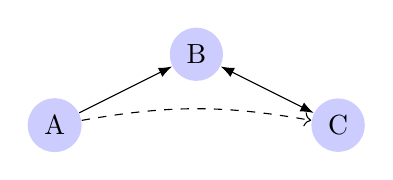
\begin{tikzpicture}  
  [scale=.9,auto=center,every node/.style={circle,fill=blue!20}] 
    
  \node (a1) at (0,0) {A};  
  \node (a2) at (2,1)  {B}; 
  \node (a3) at (4,0)  {C}; 
  
  \path[] (a1) edge[bend left=0]  (a2); 
  \path[bidirected] (a2) edge[bend left=0]  (a3);
  \path[dashed,->] (a1) edge[bend left=10]  (a3); 
\end{tikzpicture} 
\begin{defi}
    The model has random variables $\tau$ and $\lambda$. Other parameters are constant. 
\end{defi}
Let Alice sends payment $c_{AB}$ to Bob at a rate of $\lambda_{AB}$, and Alice wants to send payments of $c_{AC}$ to Charlie at a rate of $\lambda_{AC}$. 

Bob can serve as an intermediate node for Alice such that she does not need to create a channel with Charlie. We investigate Bob's cost and fee. 
\begin{assumption}
    Bob and Charlie makes more frequent and larger payments with each other, such that Bob is not concerned about the impact Alice's payments has on the channel between him and Charlie.
\end{assumption}
Let the size of the channel $AB$ be $m$.
The net change of balance $\Delta c$ (unit: $token/tx$) for Bob on the channel $AB$ is  
\begin{align}
    \Delta c = &c_{AC}/\frac{\lambda_{AC}}{max(\lambda_{AC},\lambda_{AB})}+c_{AB}/\frac{\lambda_{AB}}{max(\lambda_{AC},\lambda_{AB})}+p/\frac{\lambda_{AC}}{max(\lambda_{AC},\lambda_{AB})}
\end{align}
\begin{assumption}
    All the channels have the same $\lambda$.
\end{assumption}
Then the number of intermediate transaction $k$ does not depend on $\lambda$. 
\begin{align}
    \Delta c& = c_{AC}+c_{AB}+p\\
    k &= \frac{m}{\Delta c_{AB}} = \frac{m}{c_{AC}+c_{AB}+p}
\end{align}

Then we find the amount of time the channel $AB$ is open in terms of $\lambda$s. 

The rate of change in balance $\Delta B$ (unit: $token/minute$) of the channel $AB$ is 
\begin{align}
    \Delta B &= c_{AC}\lambda_{AC}+c_{AB}\lambda_{AB}+p\lambda_{AC} = (c_{AC}+c_{AB}+p)\lambda
\end{align}

Hence, the time a channel is open is 
\begin{align}
    \tau = \frac{m}{\Delta B} = \frac{m}{c_{AC}\lambda_{AC}+c_{AB}\lambda_{AB}+p\lambda_{AC}}=\frac{m}{(c_{AC}+c_{AB}+p)\lambda}
\end{align}
\begin{remark}
    $\lambda$ is a random variable depended on $\tau$. However, since $\lambda$ is not involved with the later calculations, we will not calculate its value and assume that it is some appropriate function of $\tau$. 
\end{remark}

\subsection{Interest return gain in bank}

By storing $\frac{c}{e^{r\tau}}$ in the bank at time $t=0$, the balance grow to $c$ at time $t=\tau$. If a node store $c$ in the channel, then assuming they do not change the balance, then they get $c$ back when the channel closes.\\
The cost to store $c$ in a channel that opens during the time $(0,\tau)$, is 
\begin{align}
    I_1 &= c-ce^{-r\tau}
\end{align}
Then the expected interest return of a channel is 
\begin{align}
    I(\alpha) = E[I_1] &= c-cE[e^{-r\tau}] = c-c\frac{\alpha}{\alpha + r}
\end{align}

\subsection{Transaction fee}
Recall the number of transactions Bob can handle is $k = \frac{m}{\Delta c}=\frac{m}{c+c_{AB}+p}$. 
\begin{assumption}
    Bob charges a constant fee $p$ for each transaction
\end{assumption}
For the entirety of the channel, Bob will gain transaction fee
\begin{align}
    T_1 = p\cdot k \cdot e^{-r\tau}
\end{align}

Then the expected gain is 
\begin{align}
    T(\alpha) &= E[T_1] = p\cdot k \cdot E[e^{-r\tau}]\\
    & = \frac{mp}{c_{AC}+c_{AB}+p} \cdot \frac{\alpha}{\alpha + r}
\end{align}

\end{document}